\section{Simulation result}

This section present the simulation result based on the feedback-based congestion control. To simplify the problem. I start from a small network just contain single core router but with multiple edge routers. And then go through a normal network. The result demonstrated that congestion control police can reduce burst block ratio and prevent network from entering congestion status.

\begin{table}[!htb]
\renewcommand{\arraystretch}{1.3}
\caption{Common Parameter}
\label{tab:cp}
\centering
\begin{tabular}{l l}
\toprule
Parameter & Value \\
\midrule
Average Burst Length & 0.0001s \\
Number of Link Wavelengths & 10 \\
Use FDLs for Ingress Bursts     & no \\
Offset time & 0.0001s\\
Signaling and scheduling mechanisms & LAUC-AF \\
Weighted factor $\alpha$  & 0.5\\
Congestion detect period & 0.2 \\
Simulation Run Length & 5s \\
\bottomrule
\end{tabular}
\end{table}

Table \ref{tab:cp} show the common key parameters share with two scenarios. I also assume the inter-arrival time and burst service time of burst meet the exponential distribution. 

\subsection{Single node scenario}

\begin{figure}[!htb]
\centering
\includegraphics[width=2.6in]{fig/single_node_topo}
\caption{Single Node Network Model}
\label{fig:sn_topo}
\end{figure}

%\hspace{1pt}

Figure \ref{fig:sn_topo} shown the single node scenario topology and the routing table is shown below:

$$\begin{vmatrix}  
 1, & 4, & 1, & 0.5, & 1, & 0, & 4 \\  
 1, & 5, & 1, & 0.5, & 1, & 0, & 5 \\  
 1, & 6, & 1, & 0.5, & 1, & 0, & 6 \\  
 2, & 4, & 1, & 0.5, & 2, & 0, & 4 \\  
 2, & 5, & 1, & 0.5, & 2, & 0, & 5 \\  
 2, & 6, & 1, & 0.5, & 2, & 0, & 6 \\  
 3, & 4, & 1, & 0.5, & 3, & 0, & 4 \\  
 3, & 5, & 1, & 0.5, & 3, & 0, & 5 \\  
 3, & 6, & 1, & 0.5, & 3, & 0, & 6 \\  
\end{vmatrix}$$

The format of each row is:
\par
{\tt \{src, dest, svc\_level, load, path\}}

So there are nine paths. Every path pass through the single core node. For comparison purpose, I evaluate the performance of without congestion control mechanism and that employ feedback-based congestion control. Before us begin, we need to define some terms:

Network Load Scale: Specifies scaling factor for traffic offered to network. Each source generate rate calculate as (Network Load Scale) x (normalised load value) x (Link Wavelengths) / (Average Burst Length).

Burst block rate: average rate of data bursts that are blocked due to fail to schedule without available channel. 

Throughput: average rate of data bursts that are successfully transfer from source node to destination node.

\begin{figure}[!htb]
\centering
\includegraphics[width=2.6in]{result/single_node/block_rate_avg}
\caption{Burst Block Rate}
\label{fig:sn_block_rate}
\end{figure}

The burst block rate trend with the network load factor which start from 0.1 to 1.0 is show in the figure \ref{fig:sn_block_rate}. To the case without congestion control mechanism, the burst block rate keeps linearly increasing with the network load factor. When reach the bottleneck capacity of network, all arriving bursts will be blocked without any control. The performance would be reduced and network resource will be wasted. The case with congestion control and congestion threshold as 0.06
achieve the lowest burst blocked rate. Since the data burst inject into network will be limited at a lower rate. The figure shown the burst block rate also increases with network load factor. The ideal result will stay a certain value. This because of the simulation time is a little short. If it last longer, the shape of line would trend to be a horizontal line.

\begin{figure}[!htb]
\centering
\includegraphics[width=2.6in]{result/single_node/throughput_avg}
\caption{Throughput}
\label{fig:sn_throughput}
\end{figure}

Figure \ref{fig:sn_throughput} compares the throughput of some case. As it illustrated, the throughput of case without congestion control gain the highest throughput. However, the growth of throughput is the expense of a highest burst block rate as shown in figure \ref{fig:sn_block_rate}. When network don't enter congestion, the throughput increase with the growth of network load scale. But if network is saturated, the throughput doesn't increase any more. The excess burst have to burst. This
figure also tell that the higher congestion threshold. Network can get higher throughput with higher blocking probability. Throughput and blocking probability trade-off should be consider.  

\begin{figure}[!htb]
\centering
\includegraphics[width=2.6in]{result/single_node/block_probability_trend}
\caption{Block Probability Trend with Congestion Control}
\label{fig:sn_block_probability}
\end{figure}

Figure \ref{fig:sn_block_probability} shown the effect of feedback-based mechanism with congestion threshold 0.06. When network load scale factor is 0.5, the burst blocking probability jitter around the threshold with congestion control. With the growth of network load scale factor, the initial burst blocked probability increase sharply. That is said it will take longer to clear out the congestion status. But when it enter stable state, The feedback-based congestion control
scheme will limit the number of data burst inject to network and leaky bucket on edge side will smooth the traffic. The simulation result demonstrated that the mechanism can reduce the burst blocked probability even thought the network load scale increase high.

\subsection{Network scenario}

\begin{figure}[!htb]
\centering
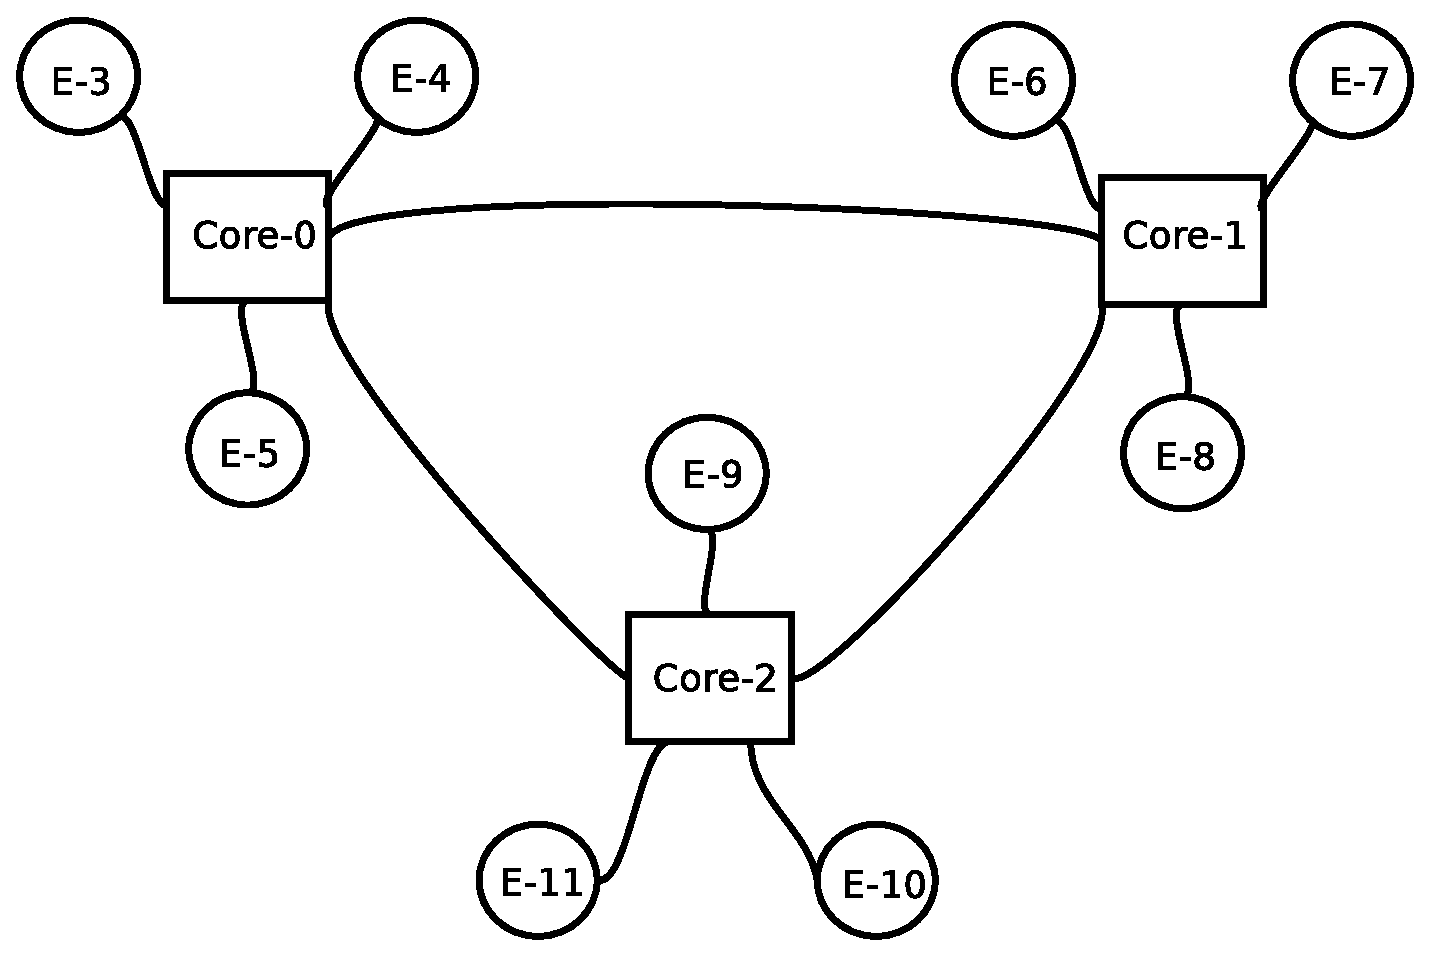
\includegraphics[width=2.6in]{fig/network_topo}
\caption{Network Model}
\label{fig:network_topo}
\end{figure}


Figure \ref{fig:network_topo} shown the network scenario topology and the routing table is shown below:

$$\begin{vmatrix}  
 3, & 6, & 1, & 0.5, & 3, & 0, & 1, & 6 \\  
 4, & 7, & 1, & 0.5, & 4, & 0, & 1, & 7 \\  
 5, & 8, & 1, & 0.5, & 5, & 0, & 1, & 8 \\  
 6, & 9, & 1, & 0.5, & 6, & 1, & 2, & 9 \\  
 7, & 10, & 1, & 0.5, & 7, & 1, & 2, & 10 \\  
 8, & 11, & 1, & 0.5, & 8, & 1, & 2, & 11 \\  
 9, & 3, & 1, & 0.5, & 9, & 2, & 0, & 3 \\  
 10, & 4, & 1, & 0.5, & 10, & 2, & 0, & 4 \\  
 11, & 5, & 1, & 0.5, & 11, & 2, & 0, & 5 \\  
\end{vmatrix}$$

There also are nine paths. However, every path pass through two core nodes. By analysing the routing table, these three core nodes are symmetrical to each others. So we just need to test if the mechanism works on any one of three core nodes. In this paper, I choose core node zero.

\begin{figure}[!htb]
\centering
\includegraphics[width=2.6in]{result/network/throughput_avg}
\caption{Throughput}
\label{fig:net_throughput}
\end{figure}

As Figure \ref{fig:net_throughput} shown, the throughput of without any control is higher than with congestion control. The reason is similar to single node scenario.

\begin{figure}[!htb]
\centering
\includegraphics[width=2.6in]{result/network/block_probability_trend}
\caption{Block Probability Trend with Congestion Control}
\label{fig:net_block_probability}
\end{figure}

Figure \ref{fig:net_block_probability} shows the burst block probability of different network load scale factor during the simulation time with congestion threshold 0.1. It demonstrate that this mechanism can reduce the burst blocked probability in network environment. The cases with different network load scale factor almost achieve the threshold level at the same time. That is said the react delay doesn't increase with the arrival rate. 


